\documentclass[11pt]{article}
%\addbibresource{references.bib}

% custom code
\usepackage[dvipsnames]{xcolor}
\definecolor{light-gray}{gray}{0.90}
\newcommand{\code}[1]{\colorbox{light-gray}{\texttt{#1}}}

\usepackage[most]{tcolorbox}
\tcbset{on line, 
        boxsep=1pt, left=1pt,right=1pt,top=1pt,bottom=1pt,
        colframe=white,colback=light-gray,  
        highlight math style={enhanced}
        }

\usepackage{tikz}
\def\checkmark{\tikz\fill[scale=0.4](0,.35) -- (.25,0) -- (1,.7) -- (.25,.15) -- cycle;}  %checkmark

% images
\usepackage{graphicx}
\graphicspath{ {./img/} }

% background
\pagecolor{white}
\usepackage[normalem]{ulem}

% bibliography
\usepackage[round]{natbib}

% additional symbols
\usepackage{amsmath}
\usepackage{amssymb}
\usepackage{gensymb}

% document links
\usepackage{hyperref}
\hypersetup{
    colorlinks,
    linkcolor={MidnightBlue!50!black},
    citecolor={MidnightBlue!50!black},
    urlcolor={MidnightBlue!80!black}
}

% tooltips
%\usepackage[inactive,blur=0.6, fixcolor]{fancytooltips}

\title{Flatland}
\author{Murphy}
\date{\today}

\begin{document}

% Title page
\maketitle	
\pagebreak

% Table of contents
\tableofcontents
\pagebreak

% Paper content

% Problem background
\section{Introduction}
\subsection{Problem Background}
The Flatland framework addresses the problem of automated train scheduling and rescheduling, a major challenge
for modern railway systems. It does so by providing a simplified two-dimensional grid world environment to allow for fast experimentation on scenarios of varying complexities \citep{monylascscbhwaegeibavistsasp20a}. 

\subsection{Related Works}
Scenarios in Flatland exist at the intersection of several well-explored problems.  At its core, Flatland is a multi-agent pathfinding problem \citep{silver05a}; several agents cooperate to complete their goals while managing limited resources within a shared, finite environment.  Outside of pathfinding, Flatland is, in essence, a vehicle scheduling problem \citep{bapeukfa00a}.  An understanding of how each of these problems influences Flatland is a critical piece of finding ideal methods of producing solutions.

\subsubsection{Multi-agent Pathfinding}
Multi-agent pathfinding (MAPF) \citep{silver05a} is a planning problem in which agents in a shared environment must find routes to their respective destinations without incurring collisions.  MAPF has many applications, including in robotics, aviation, and vehicle routing \citep{standley10a}.  Many of the conflicts imposed on agents in MAPF problems are also imposed on agents within the Flatland framework, such as that they may not occupy the same cell at the same time step, or that two agents may not swap positions.  These are to model collisions that would occur in real life.  

Traditional grid environments seen in many MAPF problems, including in \citep{standley10a}, have cells that are often four- or eight-connected; this means that an agent occupying one cell may move to any of its existing unoccupied neighboring cells.  The Flatland framework is more restrictive in this sense, as agents are not free to move indiscriminately to any unoccupied neighboring cell, but rather may move to neighboring cells according to transitions governed by the track type of that cell and the orientation of the agent at that time step, all of which is further discussed in \autoref{sec:Environment} and is illustrated more clearly in \autoref{fig:grids}.

% Figure: Grids, degrees of freedom
\begin{figure}[t]
\centering
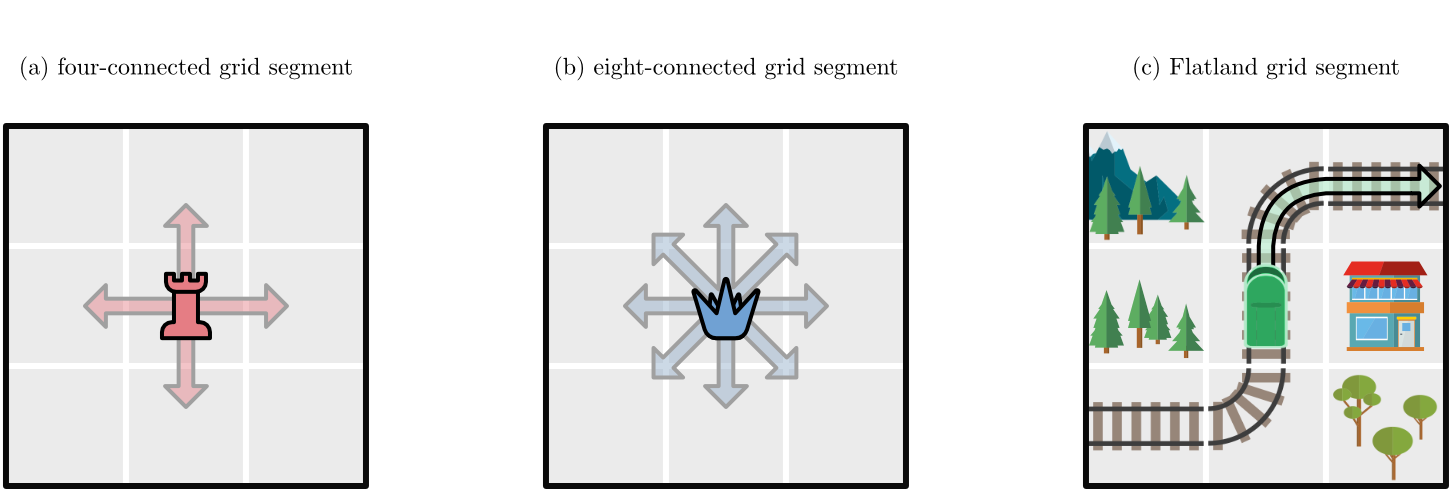
\includegraphics[width=\textwidth]{chess2}
\caption{Examples of the degrees of freedom for agents in four-connected grid environments, eight-connected grid environments, and Flatland grid environments. The red agent in grid segment (a) can move to any of its neighboring cells to the north, east, south, or west.  The blue agent in grid segment (b) can move like its red counterpart, but has additional access to diagonal neighbors as well.  The green train in the Flatland grid segment (c) is bound to the tracks.  The orientation of the agent in Flatland is necessary to determine which cells are accessible. }
\label{fig:grids}

\begin{center}
{\color{lightgray} \rule{\linewidth}{0.15mm}}
\end{center}

\end{figure}

\subsubsection{Vehicle Scheduling Problem}
The vehicle scheduling problem (VSP) \citep{bapeukfa00a} is a classical optimization problem in the field of operational planning of public transportation systems, consisting of assigning vehicles to trips, in such a way that each trip is associated to one vehicle and a cost function is minimized.  In Flatland, each instance already provides a set of agents with pairs of starting and ending positions.  However, determining the specific paths agents should follow is the problem participants are tasked with solving.  Furthermore, although not a focus of this research, Flatland provides an option to randomly inflict breakdowns upon its fleet.  When this option is selected, the task effectively extends into the realm of the vehicle rescheduling problem (VRSP) \citep{limibo07a}, as the recalculation of paths to accommodate for such breakdowns must take place once the trains have begun moving.


% Potential approaches
\section{Approaches}
AIcrowd \citep{baeiegljmomonyspwaaggo21a} hosts a global competition in which participants submit crafted approaches to scenarios in Flatland, which are scored and compared with one another.  The variety of submissions highlights the diverse nature of approaches taken to solve the problem Flatland presents.

\subsection{Reinforcement Learning}
Reinforcement learning is a form of machine learning in which an agent with a goal is not told what steps to take, but rather discovers a path to it by determining which actions yield the greatest reward \citep{sutton18a}.  This differs from \textit{supervised learning} in which agents are shown a set of labeled examples of desired outcomes so that it can generalize for unseen situations.  This also differs from \textit{unsupervised learning} in which agents seek to uncover structures or patterns within a set of unlabeled examples.  A typical reinforcement learning approach in a Flatland scenario would include many iterations of agents relying on past actions that have yielded success and exploring new actions that aim to get them closer to the goal.

Although the competition is open to approaches from any domain, it has branded itself as a competition for multi-agent reinforcement learning.  In the latest two iterations of the competition, separate leaderboards were posted for those pursuing the reinforcement learning track and those pursuing all other approaches.  Despite this focus, the highest any participant has placed with a reinforcement learning solution has been seventh place.

\subsection{Operations Research}
Operations research \citep{gupta92a} is a broader field pertaining to the application of scientific methods to problems involving the operations of a system, such as by using the theories of probability, linear programming, queuing theory, or other methods.  The winners of the 2020 competition were a team led by professors Daniel Harabor and Peter J. Stuckey of Monash University.  The team employed a prioritized planning approach to quickly find collision-free paths, and a large neighborhood search (LNS) to improve the solution quality thereafter \citep{lichzhchhastmako21a}.

In each the last two competitions, teams with operations research-focused approaches have taken the top four spots.  The winning team members from 2020 explain in \citep{lichzhchhastmako21a} why they believe reinforcement learning approaches have not produced the same level of success as other methods:
\begin{itemize}
	\item reinforcement learning approaches need to predict future deadlocks, which appears difficult to determine without directly reasoning about paths, as optimization approaches do
	\item as the density of an environment grows, the number of situations that can lead to deadlocks increases non-linearly
	\item optimization approaches rely on global planners, which have been shown to consistently outperform reinforcement learning approaches across all rounds of both the 2019 and 2020 Flatland competitions
\end{itemize}


\subsection{Answer Set Programming}
Answer set programming (ASP) \citep{lifschitz19a} is a form of declarative programming, based on the stable model semantics of logic programming, oriented toward combinatorial search problems.  ASP has wide-ranging applications in technology and science, with a particular inclination toward NP-complete problems.


The pathfinding problem that is present in Flatland scenarios is, at its core, an NP-hard search problem.  ASP presents itself as a particularly suitable approach to solving pathfinding problems in Flatland for several reasons:
\begin{itemize}
	\item as a declarative language, encodings are constructed in terms of their goals, not their intermediate steps
	\item solutions are characterized by their formalizations, emphasizing the clear correspondence of a solution to its encoding
	\item encodings can be easily adapted to changing conditions, such as by adding more agents or including additional constraints
\end{itemize}

\noindent Generally, due to its flexibility, maintainability, human readability, and verifiability, ASP lends itself well to scalable pathfinding problems. \medskip


% The problem workflow
\section{Building Blocks}
Flatland comprises a set of components that are fundamental to its ability to simulate real-world railway scenarios.  In the forefront are the environment and the agents, which form the basis of modeling how trains traverse a physical network.

Further components include the scope of observation, the presence of breakdowns, and pre-determined timetables.  However, these are not considered within the scope of this research.

\subsection{Environment}
\label{sec:Environment}
An environment in Flatland is a grid that consists of cells that are either empty or contain tracks.  A track may belong to one of nine types shown in \autoref{fig:tracks}, and may be rotated in increments of 90\degree.  Cells must be arranged in such a way that they form a network that adheres to rules of consistency, such that that each connection out of a cell must be joined by a connection of a neighboring cell \citep{baeiegljmomonyspwaaggo21a}.  Furthermore, each cell may only be occupied by a single agent at any given time step.

\subsubsection{Track Types and Transitions}
\label{sec:Track}
Flatland documentation \citep{baeiegljmomonyspwaaggo21a} considers seven track types, however, two of them have alternative representations that are recognized as individual types in their own right, bringing the total to nine.  There is also a separate designation for an empty cell.

% Figure: Grids, degrees of freedom
\begin{figure}[t]
\centering
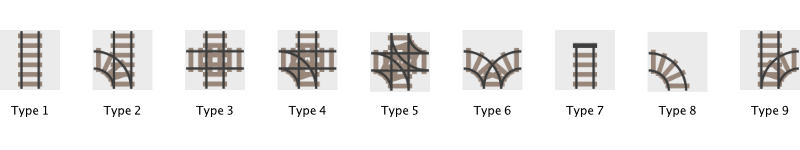
\includegraphics[width=\textwidth]{tracks}
\caption{Visual representation of all available track types.  Each type may be rotated in increments of 90\degree.  Type 8 and Type 9 are variations on Type 1 and Type 2, respectively, which cannot be attained through rotation alone.}
\label{fig:tracks}

\begin{center}
{\color{lightgray} \rule{\linewidth}{0.15mm}}
\end{center}

\end{figure}

The various rail types can be grouped into two categories: non-switches and switches.  Non-switches include tracks such as straight tracks, curved tracks, and dead ends.  These tracks do not allow an agent to make a navigation decision, meaning that on such tracks, agents are restricted to moving forward, coming to a stop, or turning around.  Conversely, switches represent decision points, as they compel agents to choose between alternative transitions, such as traveling to the left or to the right.  A switch never presents more than two options.

Each rail type determines the possible legal transitions for the agents, meaning which neighboring cells are accessible positions following a single move.  A neighboring cell is any physically adjacent cell one unit to the north, east, south, or west.  Crucially, neighboring cells that are accessible from one location, may in some cases not be accessible had the train approached this same location from another direction.  This is a fundamental underlying characteristic of Flatland.  For this reason, recording both the position and orientation of each agent at every time step is necessary for determining its legal paths.  A diagram explaining this quality is shown in \autoref{fig:transitions}.

% Figure: Grids, degrees of freedom
\begin{figure}[t]
\centering
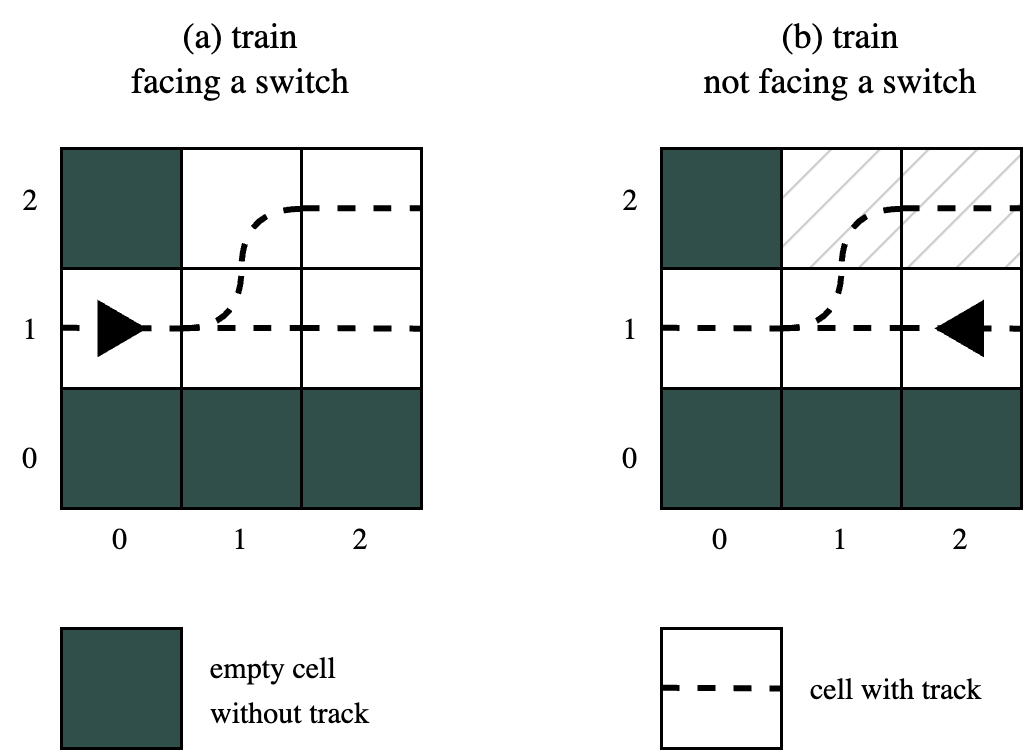
\includegraphics[width=\textwidth]{transitions}
\caption{The siding track up north is only accessible via the switch from one direction.  The switch is shown in the dashed box.  In environment (a), the red agent is traveling from the west.  When it reaches the switch, it will have the option to continue moving to the east or follow the switch into the siding.  In environment (b), the blue agent is traveling from the east and does not have access to the siding.  Therefore, when it reaches the switch, it will have to continue moving to the west.}

\begin{center}
{\color{lightgray} \rule{\linewidth}{0.15mm}}
\end{center}

\label{fig:transitions}
\end{figure}



\subsubsection{Points of Interest}
Cities and train stations are effectively synonymous in Flatland.  Cities are esthetic regions of the environment that host stations; stations are designated track cells that represent potential starting or ending points for trains.  Trains must start and end their journeys at train stations.  A single train station may have multiple tracks passing through it, in which case a train with some city as a destination may successfully reach it via any of the tracks of its train station. \medskip

\subsubsection{Generating New Environments}
\noindent The Flatland framework offers several parameters when generating novel environments.  Among others, the \tcbox{\textcolor{WildStrawberry}{\texttt{sparse\_rail\_generator}}} allows users to specify:
\begin{itemize}
	\item the environment size
	\item the number of trains
	\item the number of cities
	\item the number of connections between cities
\end {itemize}


\subsection{Agents}
\label{sec:Agents}
Agents in Flatland represent the trains of a railway network.  At any time step, each agent can perform one of four unique actions, is given a starting location and specified destination, and must avoid collisions and other conflicts with agents present throughout the environment.  The primary goal of an agent is to follow a path from its origin to its destination without incurring a collision.  The terms \textit{agent} and \textit{train} are used interchangeably.

Additionally, agents in Flatland may have different speeds, depending on their train types, such as passenger trains or freight trains.  This speed profile determines how quickly agents are capable of traversing the environment, and ultimately influences how they interact with one another.  For simplicity, the scope of this research recognizes only a uniform speed profile and does not distinguish between train types.  Trains in motion are capable of traversing the environment at a rate of one cell per time step \citep{baeiegljmomonyspwaaggo21a}.

\subsubsection{Actions}
\label{sec:Actions}
Within the environment, agents follow a series of actions.  Flatland is a discrete time simulation, and the duration of each action conforms to a constant amount of time.    At each time step, agents must choose from one of the following four actions, provided there is a legal transition: 
\begin{enumerate}
  \item \tcbox{\textcolor{WildStrawberry}{\texttt{MOVE\_FORWARD}}}: along a straight track, this action moves the train forward; over a switch, this action moves the train along the straight edge; along non-switch curved track, this action moves the train along the curve; in dead ends, this reverses the direction of the train
  \item \tcbox{\textcolor{WildStrawberry}{\texttt{MOVE\_LEFT}}}: this action moves the train along the left edge of a switch
  \item \tcbox{\textcolor{WildStrawberry}{\texttt{MOVE\_RIGHT}}}: this action moves the train along the right edge of a switch
   \item \tcbox{\textcolor{WildStrawberry}{\texttt{STOP\_MOVING}}}: this action stops the train in its current cell
\end{enumerate} \smallskip

\noindent So long as a valid action has been selected, the position and orientation of the agent will be updated in the following time step.  A fifth action in Flatland, \tcbox{\textcolor{WildStrawberry}{\texttt{DO\_NOTHING}}}, is ignored as it is superfluous and any Flatland solution can be executed without using this action.  \medskip

\begingroup

\setlength{\tabcolsep}{9pt} % Default value: 6pt
\renewcommand{\arraystretch}{1.2} % Default value: 1

\begin{table}[]
\centering
\begin{tabular}{rcccc}
						& $ \Lsh  $ 	& 			& $ \Rsh  $ 	& $\curvearrowright$ \\
                                      		& -90\degree 	& 0\degree 	& 90\degree 	& 180\degree \\

\hline % ————————————————————————————————————————
\texttt{MOVE\_FORWARD} 	& \checkmark  	& \checkmark 	& \checkmark  	& \checkmark \\
\texttt{MOVE\_LEFT}    		& \checkmark 	& 			& 			& \\
\texttt{MOVE\_RIGHT}   		& 			& 			& \checkmark 	& \\
\texttt{STOP\_MOVING}  		& 			& \checkmark 	& 			& 
\end{tabular}
\caption{How each action can change the orientation of an agent in the following time step.  A change of 0\degree is analogous to no change.}
\label{tbl:actions}
\begin{center}
{\color{lightgray} \rule{\linewidth}{0.15mm}}
\end{center}
\end{table}


\endgroup


As shown in \autoref{tbl:actions}, different actions are capable of affecting subsequent agent orientation in various ways.  When on a non-curved track, \tcbox{\textcolor{WildStrawberry}{\texttt{MOVE\_FORWARD}}} imposes is no change on the agent orientation in the following time step.  When on curved track (Type 9 in \autoref{fig:tracks}) this action can rotate the agent by 90\degree counterclockwise or clockwise, depending on the direction of the curve.   When in a dead end (Type 7 in \autoref{fig:tracks}), this action reverses its direction, rotating the agent by 180\degree .  \tcbox{\textcolor{WildStrawberry}{\texttt{MOVE\_LEFT}}} and \tcbox{\textcolor{WildStrawberry}{\texttt{MOVE\_RIGHT}}} are valid actions for switches and always alter the current orientation of the agent by 90\degree counterclockwise or clockwise, respectively.  \tcbox{\textcolor{WildStrawberry}{\texttt{STOP\_MOVING}}} never alters the current orientation of the agent.

\subsubsection{Starting and Ending Positions}
\label{sec:Positions}
Each agent is given a starting position and orientation, as well as a destination.  The goal for a single agent is to traverse the environment by choosing valid actions along legal paths that lead the agent from its starting position to its destination.  

For simplicity, trains are not recognized by the environment until they are actively underway.  This prevents trains who have not yet begun their journeys from occupying space on the tracks and preventing the passage of other trains.  Likewise, once a train reaches its destination, it is no longer recognized as actively being present in the environment.  The track space therefore becomes free in the time step after the train has completed its journey.

\subsubsection{Conflict Restrictions}
\label{sec:Conflicts}
Consistent with core tenets of any MAPF problem, any two trains must avoid a collision with each other.  Agents, as with trains in real life, may not physically pass through one another.  This restriction prevents one train from overtaking a stopped train on the same set of tracks; it also prevents two trains facing each other from swapping positions.

\bibliographystyle{plainnat}
\bibliography{references}
\end{document}
